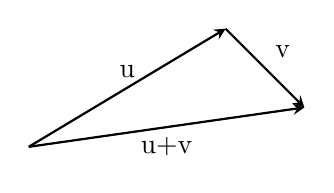
\begin{tikzpicture}
\coordinate(N1) at (-3.5,68) {} {} {} ;
\coordinate(N2) at (-1,69.5) {} {} {};
\coordinate(N3) at (0,68.5) {} {} {} {} ;
\draw[-stealth,thick](N1)--node[pos=.5,above ] {u}(N2);
\draw[-stealth,thick](N1)--node[pos=.5,below ] {u+v}(N3);
\draw[-stealth,thick](N2)--node[pos=.5,above right] {v}(N3);
\end{tikzpicture}